%% ****** Start of file apstemplate.tex ****** %
%%
%%
%%   This file is part of the APS files in the REVTeX 4 distribution.
%%   Version 4.1r of REVTeX, August 2010
%%
%%
%%   Copyright (c) 2001, 2009, 2010 The American Physical Society.
%%
%%   See the REVTeX 4 README file for restrictions and more information.
%%
%
% This is a template for producing manuscripts for use with REVTEX 4.0
% Copy this file to another name and then work on that file.
% That way, you always have this original template file to use.
%
% Group addresses by affiliation; use superscriptaddress for long
% author lists, or if there are many overlapping affiliations.
% For Phys. Rev. appearance, change preprint to twocolumn.
% Choose pra, prb, prc, prd, pre, prl, prstab, prstper, or rmp for journal
%  Add 'draft' option to mark overfull boxes with black boxes
%  Add 'showpacs' option to make PACS codes appear
%  Add 'showkeys' option to make keywords appear
\documentclass[aps,prl,twocolumn,superscriptaddress]{revtex4-1}
%\documentclass[aps,prl,preprint,superscriptaddress]{revtex4-1}
%\documentclass[aps,prl,reprint,groupedaddress]{revtex4-1}

% You should use BibTeX and apsrev.bst for references
% Choosing a journal automatically selects the correct APS
% BibTeX style file (bst file), so only uncomment the line
% below if necessary.
\bibliographystyle{apsrev4-1}
%\usepackage{cite}

%\usepackage[english]{babel}
%\usepackage[utf8]{inputenc}
\usepackage{amsmath}
\usepackage{graphicx}
\usepackage{amsfonts}
%\usepackage[colorinlistoftodos]{todonotes}

\usepackage[caption=false]{subfig}
%\usepackage{graphicx}
%\usepackage{caption}
%\usepackage{subcaption}
\newcommand{\vcrm}[1]{\mathbf{#1}}
\newcommand{\hvcrm}[1]{\mathbf{\hat{#1}}}
\newcommand{\vc}[1]{\boldsymbol{#1}}
\newcommand{\hvc}[1]{\boldsymbol{\hat{#1}}}

\newcommand{\ssa}[0]{\sin{\alpha}}
\newcommand{\cca}[0]{\cos{\alpha}}
\newcommand{\ssb}[0]{\sin{\beta}}
\newcommand{\ccb}[0]{\cos{\beta}}
\newcommand{\ssc}[0]{\sin{\gamma}}
\newcommand{\ccc}[0]{\cos{\gamma}}
\newcommand{\sst}[0]{\sin{\theta}}
\newcommand{\cct}[0]{\cos{\theta}}
\newcommand{\ssp}[0]{\sin{\phi}}
\newcommand{\ccp}[0]{\cos{\phi}}

\newcommand{\xsa}[0]{\sin{\alpha}}
\newcommand{\xca}[0]{\cos{\alpha}}
\newcommand{\xsb}[0]{\sin{\beta}}
\newcommand{\xcb}[0]{\cos{\beta}}
\newcommand{\xsc}[0]{\sin{\gamma}}
\newcommand{\xcc}[0]{\cos{\gamma}}
\newcommand{\xst}[0]{\sin{\theta}}
\newcommand{\xct}[0]{\cos{\theta}}
\newcommand{\xsp}[0]{\sin{\phi}}
\newcommand{\xcp}[0]{\cos{\phi}}

\newcommand{\dd}{\mathrm{d}}
\newcommand{\ee}{\mathrm{e}}
\newcommand{\ii}{\mathrm{i}}
\newcommand{\kk}{\mathrm{k}_B}

\newcommand{\vm}{\vc{\mu}}
\newcommand{\vn}{\hvcrm{n}}
\newcommand{\vB}{\vcrm{B}}
\newcommand{\vz}{\hvcrm{z}}


\begin{document}

% Use the \preprint command to place your local institutional report
% number in the upper righthand corner of the title page in preprint mode.
% Multiple \preprint commands are allowed.
% Use the 'preprintnumbers' class option to override journal defaults
% to display numbers if necessary
%\preprint{}

%Title of paper
\title{The entropy-driven orientational hopping of a magnetically confined colloidal rod arises from a thermal analogue of gimbal lock}

% repeat the \author .. \affiliation  etc. as needed
% \email, \thanks, \homepage, \altaffiliation all apply to the current
% author. Explanatory text should go in the []'s, actual e-mail
% address or url should go in the {}'s for \email and \homepage.
% Please use the appropriate macro foreach each type of information

% \affiliation command applies to all authors since the last
% \affiliation command. The \affiliation command should follow the
% other information
% \affiliation can be followed by \email, \homepage, \thanks as well.
\author{Yongxiang Gao}
\affiliation{Department of Chemistry, Physical and Theoretical Chemistry Laboratory, University of Oxford}
\author{Andrew Kaan Balin}
\affiliation{The Sir Rudolf Peierls Centre for Theoretical Physics, University of Oxford}
\author{Roel P.A.\ Dullens}
\affiliation{Department of Chemistry, Physical and Theoretical Chemistry Laboratory, University of Oxford}
\author{Julia M.\ Yeomans}
\affiliation{The Sir Rudolf Peierls Centre for Theoretical Physics, University of Oxford}
\author{D.G.A.L.\ Aarts}
\affiliation{Department of Chemistry, Physical and Theoretical Chemistry Laboratory, University of Oxford}
%\email[]{Your e-mail address}
%\homepage[]{Your web page}
%\thanks{}
%\altaffiliation{}


%Collaboration name if desired (requires use of superscriptaddress
%option in \documentclass). \noaffiliation is required (may also be
%used with the \author command).
%\collaboration can be followed by \email, \homepage, \thanks as well.
%\collaboration{}
%\noaffiliation

\date{\today}

\begin{abstract}
We report the counter-intuitive behaviour of a passive colloidal ferromagnetic rod under the influence of a static external magnetic field. The sedimented rod periodically switches from a low energy horizontal state to a substantially high energy vertical state at no reduction of magnetic potential energy. We provide a thorough statistical mechanical analysis of the system by deriving the Boltzmann distribution across rod orientations which shows that switching on the magnetic field leads to the emergence of a metastable vertical state; the histogram of angle data is in good qualitative agreement with the analytic probability distribution ---both show a probability-minimum at an intermediate angle somewhere between the vertical and horizontal orientations. We show that this is an entirely entropic process that results from the loss of degree-of-freedom (and associated gain in explorable phase space) that occurs when two axes of rotation coincide ---an effect known in classical mechanics as gimbal lock.\end{abstract}

% insert suggested PACS numbers in braces on next line
\pacs{}
% insert suggested keywords - APS authors don't need to do this
%\keywords{}

%\maketitle must follow title, authors, abstract, \pacs, and \keywords
\maketitle

%%%%%%%%%%%%%%%%%%%%%%%%%%%%%%%%%%%%%%%%%%%%%%%%%%%%%%%%%%%%%%%%%%%%
%
%
%
%
%					I N T R O D U C T I O N
%
%
%
%%%%%%%%%%%%%%%%%%%%%%%%%%%%%%%%%%%%%%%%%%%%%%%%%%%%%%%%%%%%%%%%%%%%
%\section{Introduction}
\emph{Introduction.} In soft matter, many phenomena are governed by entropy. Examples include: polymer translocation through microchannels \cite{Muthukumar1989,Ledesma-Aguilar2012}, accumulation of colloidal spheres at corners of a rough substrate \cite{Dinsmore1996} and particle diffusion through constrictive environments or around obstacles \cite{Chou1999,Zwanzig1992}. Understanding such phenomena is key in the manufacturing of microscopic devices whose functioning must often either defeat or exploit the thermal nature of the environment they reside in. Devices controlled or actuated by external fields ---be it magnetic, electric or gravitational--- have a great potential to find applications in emerging nanotechnologies. It has been suggested that novel self-folding nanowire which respond to magnetic fields can be implemented in minimally invasive surgery \cite{Xi2013,Solovev2012}. Other utilities for actuated microscopic devices include the pumping or mixing of fluids \emph{[citation]}, self-propulsion \emph{[citation]} and active transport of colloids \emph{[citation]}. One of the central goals of this type of engineering is to be able to understand how the complex rheology, dynamics or collective behaviour emerges out of the equilibrium single-particle properties. This can be especially difficult when they are expected to operate in confined geometries such as blood vessels, microfluidic channels, or porous media. 

In this letter, we demonstrate unexpected hopping behaviour of a passive ferromagnetic nanorod under the influence of a static external magnetic field. The rod is observed to transit between horizontal and vertical orientations with respect to the sedimentation plane, despite the latter state corresponding to an overall gain of $\sim3 \kk T$ in potential energy. Its long-time distribution of polar angles reveals two peaks at $0$ and $\phi/2$ (vertical and horizontal respectively), separated by an effective barrier. This system is simple enough to yield a full analytical description with no adjustable parameters, revealing the entropic nature of this behaviour.  

\begin{figure}
		\includegraphics[width=0.88\columnwidth]{figs/geometry.pdf}
	\caption{\footnotesize \emph{Main:} Geometry and notation used throughout. The orientation of the rod, $\hvcrm{n}$ is defined as the unit vector pointing along the long axis of the rod in the $+$ve $z$-direction. This makes an angle $\theta$ with the $z$-axis and its projection in the $xy$-plane subtends an angle $\phi$ with the $x$-axis. A perpendicular permanent magnetic moment $\vc{\mu}$ is embedded in one of the caps and rotates rigidly with the rod. An external magnetic field $\vcrm{B}$ is applied in the $x$-direction while the gravitational field acts in the $-$ve $z$-direction. \emph{Inset:} Euler angles are useful for describing the fixed-body rotation of the rod, where $\hvcrm{n}=\hvcrm{z}'$, $\vc{\mu}=\mu\hvcrm{x}'$, $\beta=\theta$, and $\alpha=\phi+\frac{\pi}{2}$.\label{fig:geometry}}
\end{figure}


\emph{Methods.} We grew silica particles in the shape of hemispherically capped cylinders with total length measured to be $L \approx 3.5  \mu$m and diameter $d \approx 0.65 \mu$m ---for the detailed protocol, see the Supplementary Information. Each rod was doped with magnetite (Fe$_3$O$_4$) nanoparticles in one of the hemispherical caps. Upon application of a strong external magnetic field \emph{[$B=$?]}, the caps would acquire a net magnetization $\vc{\mu}$ in the cross-sectional plane of each rod (i.e.\ perpendicular to the rods' long-axis). These particles were suspended in DI water (Millipore, 18.2 M$\Omega$) at a very low volume fraction (\sim 10^{-6}$) and were loaded into a custom glass cell (inner dimension $2\times0.5\times0.15$ cm$^3$). We let the sample sit on the microscope stage for 10 minutes, allowing adequate time for the particles to sediment. An external magnetic field was applied by a pair of Helmholtz coils with an approximate range of $0$-$150$ G. All experiments were conducted at room temperature on an inverted light microscope (Olympus IX73) equipped with a $60X$ oil-immersion lens (NA=1.42). Bright field images were acquired at 20 frames per second by a Ximea digital camera. 

Figure \ref{fig:geometry} shows a schematic representation of a typical rod synthesised using the above process, as well as the coordinate system we use to describe its orientation. The long axis of the rod is spanned by $\hvcrm{n}$ which in the laboratory frame makes an angle $\theta$ with the $z$-axis, and an angle $\phi$ in the $xy$-plane. One cap of the rod has embedded in it a permanent magnetic moment $\vc{\mu}$ that is perpendicular to $\hvcrm{n}$ and requires a third angle, $\gamma$, to parameterise its direction in the cross-sectional plane of the rod. If we consider the fixed-body coordinates of the rod, $(x',y',z')$, then $\hvcrm{n}$ lies along the $z'$-axis, $\vc{\mu}$ lies along the $x'$-axis, and the conventional $Z_\alpha X_\beta Z_\gamma$ Euler angles $(\alpha=\phi+\pi/2, \beta=\theta, \gamma)$ describe the rotation of the rod-frame relative to the lab-frame. Henceforth we shall only use $(\phi,\theta,\gamma)$ to enumerate the states of the rod. 

%\begin{figure}
%	\begin{subfigure}[b]{0.48\columnwidth}
 %   	\includegraphics[width=\textwidth]{figs/Figure2a.eps}
  %  	\caption{}
   % \end{subfigure}
    %\begin{subfigure}[b]{0.48\columnwidth}
    %	\includegraphics[width=\textwidth]{figs/Figure2b.eps}
    %	\caption{}
    %\end{subfigure}
    %\caption{\footnotesize (a) Probability distribution of the azimuthal angle of deviation $\phi-\phi_0$ of the rod from alignment with a static magnetic field. The data appear to be distributed normally with a spread $\langle \phi^2 \rangle$ obtained by applying a Gaussian fit. (b) The equipartition theorem states $\frac{1}{2} k_\phi \langle \phi^2 \rangle = \frac{1}{2}\kk T$ where $k_\phi =\mu B$ is the stiffness of the torsional trap. We make use of this to show that $\kk T / \langle \phi^2 \rangle $ increases linearly with $B$, in other words, $\mu$ remains constant (see inset) across the range of field strengths used.\label{fig:trap}}
	%\label{fig:moment}
%\end{figure}

\begin{figure}
	\centering
	\subfloat[][]{\includegraphics[width=0.25\textwidth]{figs/Figure2a.eps}} 
	\subfloat[][]{\includegraphics[width=0.25\textwidth]{figs/Figure2b.eps}}
	\caption{\footnotesize (a) Probability distribution of the azimuthal angle of deviation $\phi-\phi_0$ of the rod from alignment with a static magnetic field. The data appear to be distributed normally with a spread $\langle \phi^2 \rangle$ obtained by applying a Gaussian fit. (b) The equipartition theorem states $\frac{1}{2} k_\phi \langle \phi^2 \rangle = \frac{1}{2}\kk T$ where $k_\phi =\mu B$ is the stiffness of the torsional trap. We make use of this to show that $\kk T / \langle \phi^2 \rangle $ increases linearly with $B$, in other words, $\mu$ remains constant (see inset) across the range of field strengths used.\label{fig:trap}}
\end{figure}



\emph{Results.} Due to its large density relative to water, ($\Delta\rho = \rho_r - \rho_w \approx 0.9 \cdot 10^3$ kgm$^{-3}$) a rod undergoes fast sedimentation on the coverslip of the microscope slide and will naturally lie horizontally in the plane ($\theta\lesssim\pi/2$) whilst undergoing rotational Brownian motion in $\phi$ when no external field is present. Thermal deviation far below $\theta=\pi/2$ is heavily suppressed by gravity. In the presence of an in-plane magnetic field $\vcrm{B}=B\hvcrm{x}$, the magnetic moment $\vc{\mu}$ aligns with $\vcrm{B}$, trapping the rod in the $yz$-plane. The azimuthal angle of the rod fluctuates about either the points $\phi_0=\pm\pi/2$. We make use of the equipartition theorem $\langle -\vc{\mu}\cdot\vcrm{B}\rangle = \frac{1}{2}\mu B \langle \Delta\phi^2 \rangle = \frac{1}{2}\kk T$ to calculate the strength of the moment $\mu$ by measuring the fluctuations $\Delta\phi=\phi-\phi_0$ at varying field strengths at room temperature. The assumption we make here is that for small deviations from $\phi_0$, the rod experiences an approximately \emph{Hookean} torque: $|\tau| = k_\phi \sin{\Delta\phi}\approx k_\phi\Delta\phi$, which gives rise to the quadratic energy $U_B=\frac{1}{2}k_\phi \Delta\phi^2$ with spring constant given by $k_\phi=\mu B$. Figure \ref{fig:trap} shows that the spread of $\Delta\phi$ decreases for larger $B$, and does so in a manner whereby $\mu(B)$ remains constant across the full range of fields applied, from which we infer that the rod cap is ferromagnetic. With these results we were able to measure the strength of the moment of each rod. Typically, we found their magnitude to be approximately $1-2 \ \kk T$G$^{-1}$ \emph{[error?]} at room temperature. For the subsequent experiments, we used a rod with a moment strength measured to be $\mu = 1.2\pm0.1\ \kk T$G$^{-1}$.

\begin{figure}
%\begin{subfigure}[t]{0.31\columnwidth}
%    	\includegraphics[width=\textwidth]{figs/Figure3bb}
%    	\caption{\label{horizontal}}
%    \end{subfigure}
%	\begin{subfigure}[t]{0.31\columnwidth}
%    	\includegraphics[width=\textwidth]{figs/Figure3ba}
%    	\caption{\label{vertical}}
%    \end{subfigure}
%    \begin{subfigure}[t]{0.32\columnwidth}
%    	\includegraphics[width=\textwidth]{figs/Figure3bc}
%    	\caption{\label{timeseries}}
%    \end{subfigure}
%    \begin{subfigure}[b]{0.48\columnwidth}
%    	\includegraphics[width=\textwidth]{figs/Phi_vs_L_0G.eps}
%    	\caption{$B = 0$ G \label{Pxy_data}}
%    \end{subfigure}
%    \begin{subfigure}[b]{0.48\columnwidth}
%    	\includegraphics[width=\textwidth]{figs/Phi_vs_L_140G.eps}
%    	\caption{$B = 140$ G \label{Pxy_data2}}
%    \end{subfigure}
%    \begin{subfigure}[b]{0.98\columnwidth}
%    	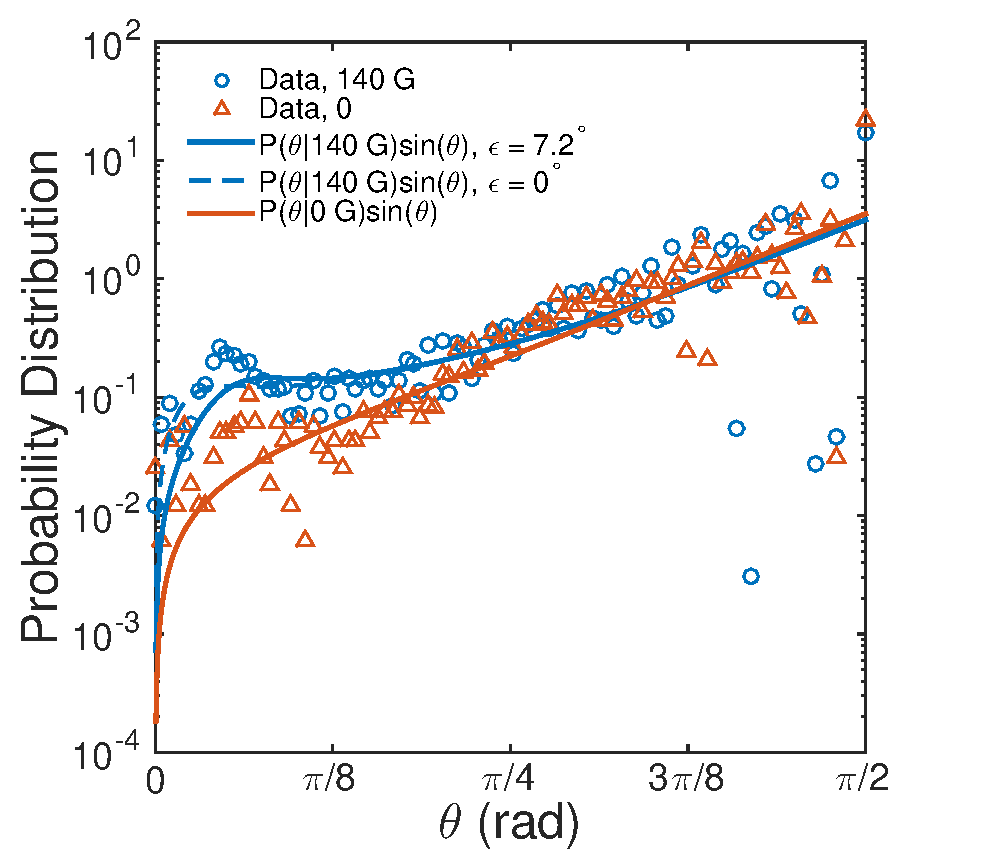
\includegraphics[width=\textwidth]{figs/Figure3a.eps}
%    	\caption{\label{Pdata}}
%    \end{subfigure}
\centering
\subfloat[][]{\includegraphics[width=0.3\columnwidth]{figs/Figure3bb}\label{horizontal}}
\subfloat[][]{\includegraphics[width=0.3\columnwidth]{figs/Figure3ba}\label{vertical}}
\subfloat[][]{\includegraphics[width=0.3\columnwidth]{figs/Figure3bc}\label{timeseries}} \\
\subfloat[][$B = 0$ G]{\includegraphics[width=0.5\columnwidth]{figs/Phi_vs_L_0G.eps}\label{Pxy_data}}
\subfloat[][$B = 140$ G]{\includegraphics[width=0.5\columnwidth]{figs/Phi_vs_L_140G.eps}\label{Pxy_data2}} \\
\subfloat[][]{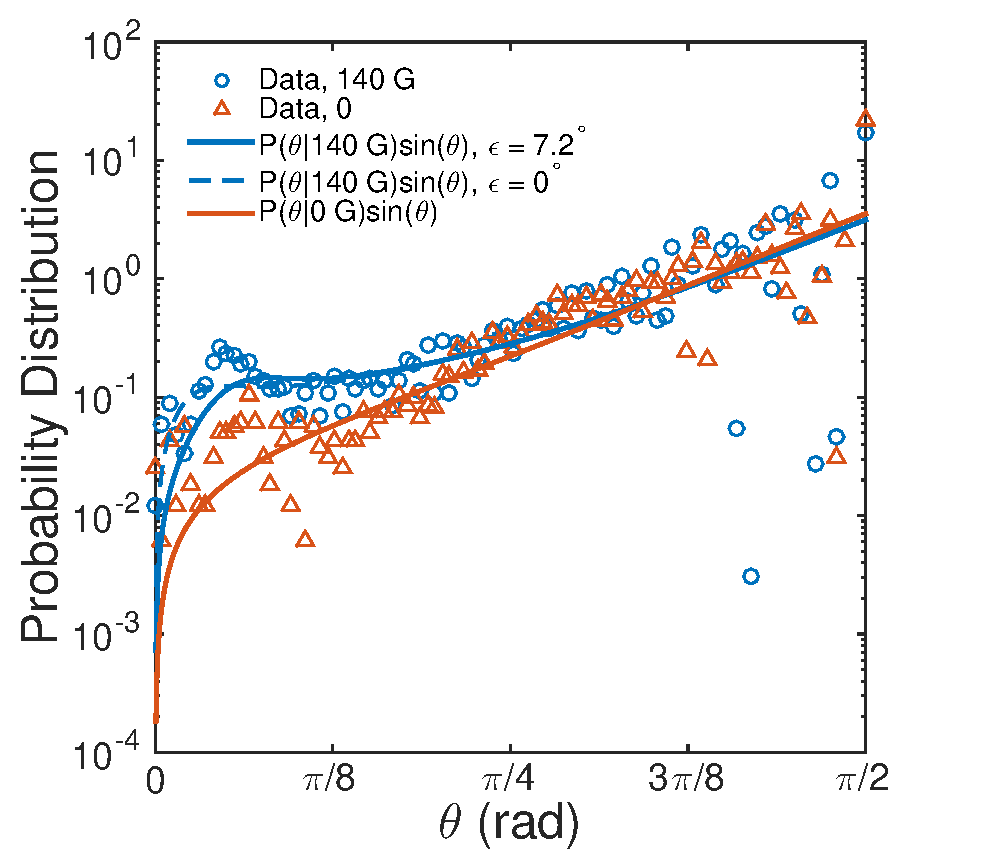
\includegraphics[width=\columnwidth]{figs/Figure3a.eps}\label{Pdata}}
    \caption{\footnotesize (a-b) A magnetic field in the $x$-direction is responsible for the trapping of the rod in the $yz$-plane; we observe the rod to hop between two states: (a) horizontally along $\pm x$ with $\theta=\pi/2$, and (b) vertically along $z$, where $\theta=0$. (c) A short segment of projected length $L_p(t)$ demonstrates the `hopping' nature of this behaviour. (d-e) The distributions of $\theta(t)$-$\phi(t)$ data falls on top of the theoretically predicted distributions $P(\phi,\theta)|_{B=0,140\ \text{G}}$. The trapping angle of the rod $|\phi_0|=(82.8\pm0.2)^\circ < \pi/2$ suggests that the magnetic moment is not quite perpendicular to the rod, making an angle $\epsilon=(7.2\pm0.2)^\circ$ with cross-sectional plane. The radial pattern in the data is an artefact of propagating the measured projected length, $L_p$, through an inverse sine function in the calculation of $\theta$ (f) Histogram of $L_p(t)$ over 60 minutes shows a markedly increased tendency for vertical states ($L_p \approx 1 \mu$m) to be realised when a magnetic field is present (blue) with respect to a free rod, under no magnetic field (red).}
\end{figure}

The main experimental observation that motivated this study was that confinement of the rod to the $yz$-plane by a magnetic field resulted in the emergence of an apparent bistability between vertical ($\theta \approx 0$) as well as horizontal ($\theta \lesssim \pi/2$) orientations, with thermal fluctuations alone strong enough to excite both states ---in contrast to an energy consuming excitation/relaxation process. Importantly, this effect occurs in spite of the fact that the rod gains $\frac{1}{2}\Delta\rho V g \approx 3.4 \ \kk T$ of gravitational potential energy at no reduction in magnetic energy $\vc{\mu}\cdot \vcrm{B}$, thus defying intuition.


This dynamic behaviour is best described as a hopping transition between these two states, occurring at random with a characteristic forwards- and backwards-rate and is apparent in real-time video data \emph{[see Supplementary Information?]}. Two images captured at different times are displayed in Figs.\ \ref{horizontal} and \ref{vertical}. By automated analysis of the images, we measured the projected length of the rod in the $xy$-plane at each time, $L_p(t)$ ---a segment of which is shown in Fig.\ \ref{timeseries}. We also measured the azimuthal angle $\phi(t)$ of the rod in the image plane. Figure \ref{timeseries} shows clearly the hopping behaviour between the horizontal state ($L_p \approx 3.5 \mu m$) and the vertical state ($L_p \approx 1 \mu m$). We noted a difficulty in the image acquisition and subsequent analysis: the minimum projected length measured ($\sim 1\mu$m) is considerably greater than the diameter of the rod ($0.65\pm0.1\mu$m). Ideally, the projected length of a hemispherically capped cylinder should be related to the polar angle by $L_p = d + (L-d)\sin\theta$, however due to shadowing and blurring effects which are functions of $\theta$ themselves --when the rod is standing up, it is more out of focus than when it is flat-- this naive interpretation of $L_p$ as being a linear function of $\sin\theta$ breaks down. In lieu of a better model, and for the sake of simplicity, we calculated the polar angle using $\theta(t) = \sin^{-1}{[(L_p(t)- L_{p,\text{min}})/(L_{p,\text{max}}-L_{p,\text{min}})]}$, where $L_{p,\text{max}}=3.5$ and $L_{p,\text{min}}=1$, ignoring any frames $t$ in which values of $L_p(t)$ fall out of this range. As this estimation does not capture the nonlinear We are careful to avoid making quantitative comparisons of the data with the theory, but our main experimental result being qualitative in nature remains valid.

To demonstrate that the presence of a magnetic field is significantly responsible for this effect, we ran two experiments for 60 minutes $[?]$ each at $0$ G and $140$ G field strengths respectively. Figures \ref{Pxy_data} and \ref{Pxy_data2} show the results for these experiments as scatter plots of all points ($\theta(t)$,$\phi(t)$). In the absence of an external field, there is nothing to break $\phi-$symmetry, while gravity acts only to bring the rod to a horizontal orientation. In the presence of a field, however, the rod is trapped at points $\pm\phi_0$, as before. Here, we observed that rather than being trapped exactly along the $y$-axis ($\phi_0=\pi/2$), the mean azimuthal angle of the rod deviated from this by around $0.12$ rad $= 7^\circ$. This is evidence that rather than being precisely within the cross-sectional plane of the rod, $\vc{\mu}$ makes an angle $\epsilon\approx 7^\circ$ with it. In the next section, we will theoretically consider both the ideal case that $\vc{\mu}\cdot\hvcrm{n}=0$, as well as an exact description accounting for finite $\epsilon$. Figure \ref{Pdata} is a histogram of the stationary distribution of $\theta(t)$ in both cases and clearly shows how the magnetic field accounts for an $\sim O(10)$ increase in likelihood of the rod being found in the vertical state.

\emph{Theoretical Model.} Each state of the rod $(\vm,\vn)$ can be described in terms of the angles $(\phi, \theta, \gamma)$ which relate its fixed-body frame to the laboratory frame. We consider the system as an ensemble of states $(\phi,\theta,\gamma)$ with instantaneous energies $U(\phi,\theta,\gamma)$. We assume that on times much longer than the dynamical timescales, the states form a canonical ensemble. Here we ignore vertical translational freedom, assuming that there is always contact between the rod and the surface; horizontal translational motion is independent so may be factored out of our discussion entirely. These assumptions further neglect any hydrodynamic effect of the plane on the rod beyond the cutting-off the domain of $\theta$ to $[0,\pi/2]$. Under these assumptions, the total energy of the system in a given state can be written as a sum of magnetic and gravitational terms: $U = -\vm \cdot\vB + \frac{m^*l}{2} \vn \cdot \vcrm{g}$, where $m*=\Delta\rho V$ is the effective mass of the rod, and $l=L-d$ is the length of the cylindrical section. We evaluate each term in the rod's fixed body frame $(x',y',z')$, where $\vc{\mu}' :=(\mu,0,0)$ and $\hvcrm{n}' :=(0,0,1)$. The external fields in this frame are thus given by solid body rotations: $\vcrm{B}' = \vcrm{R}(\phi,\theta,\gamma)\cdot ( B \hvcrm{x})$, and $\vcrm{g}'= \vcrm{R}(\phi,\theta,\gamma)\cdot ( -g \hvcrm{z})$, where $\vcrm{R}(\phi,\theta,\gamma)$ is the rotation matrix describing the laboratory- to rod-frame transformation. It can be shown [\emph{In S.I? inc.\ def.\ R()}] that

\begin{eqnarray}
U(\phi,\theta,\gamma) & = & -\mu B (\ccc\ssp + \cct\ccp\ssc) \nonumber \\
&  + & \frac{m^*gl}{2} \cct.
\end{eqnarray}

Assuming that the states are Boltzmann-distributed gives us:

\begin{eqnarray}
P(\theta, \phi, \gamma)  =  \frac{1}{Z} \ee^{ -U(\phi, \theta, \gamma)/\kk T }, \\
Z  =  \int_0^{\frac{\pi}{2}} \sst\ \dd\theta \iint_{-\pi}^{\pi}\ \dd\phi\ \dd\gamma \ \ee^{ -U(\phi, \theta, \gamma)/\kk T }.
\end{eqnarray}

As $\gamma$ is not measurable via experiment, we wish to first find the marginal distribution $P(\theta,\phi)$ by integrating out the $\gamma$ dependence. To simplify the notation, we introduce the relative strength of the gravitational energy: $a=m^*gl/2 \kk T$ and magnetic energy: $b=\mu B/\kk T$. The integral may be carried out explicitly:

\begin{eqnarray}
P(\theta,\phi)  & = & \frac{\ee^{-a\cos\theta}}{Z} \int_{-\pi}^{\pi}  \dd\gamma \  \ee^{b(\ccc\ssp + \cct\ccp\ssc) }, \nonumber \\
           & = & \frac{\ee^{-a\cos\theta}}{Z}  I_0\Big( b\sqrt{1-\cos^2\phi\sin^2\theta} \Big) \label{P}
\end{eqnarray}where $I_0(x)$ is the modified Bessel function of the first kind \emph{[cite?]}. If we now allow $\vc{\mu}$ to be inclined with respect to the cross-sectional plane of the rod, then $\vc{\mu}'=\mu(\cos\epsilon,0,\sin\epsilon)$, results in two terms in the magnetic energy balanced by $\epsilon$:

\begin{eqnarray}
U(\phi,\theta,\gamma) & = & -\mu B \Big( \cos\epsilon [\ccc\ssp + \cct\ccp\ssc] \nonumber \\
& + & \sin\epsilon \cos\phi\sin\theta \Big) \nonumber \\
&  + & \frac{m^*gl}{2} \cct.
\end{eqnarray}

The resulting marginal distribution $P(\theta,\phi)$ is given thus by:

\begin{eqnarray}
P(\theta,\phi)  & = & \frac{\ee^{-a\cos\theta}}{Z} \Big\{ I_0\Big( b\cos\epsilon\sqrt{1-\cos^2\phi\sin^2\theta} \Big) \nonumber\\
& \times &  \ee^{-b \sin\epsilon \cos\phi\sin\theta}\Big\} \label{P_corrected}
\end{eqnarray}

This corrected distribution contains no adjustable parameters and is plotted as a heatmap underneath $(\theta(t),\phi(t))$ data in Figs. \ref{Pxy_data} and \ref{Pxy_data2} using experimental parameters $a=3.4$, $b=\{0,156\}$ and $\epsilon=7^\circ$. We see a good qualitative agreement between the data and theory.

We numerically integrated Eqs.\ (\ref{P}) and (\ref{P_corrected}) with respect to $\phi$, and plot the resulting distribution $P(\theta)$ in Fig.\ \ref{theorya} with the same parameters as above but for both $\epsilon=\{0^\circ,7^\circ\}$. The effect of a finite $b$ is to encourage the population of low-$\theta$ states that are otherwise gravitationally suppressed, revealing a minimum at $\theta_{\text{min}}\ne 0$. This is the same qualitative result as from the experiments. Furthermore, the calculated relative likelihood ratio $P(\theta|140$ G$)/P(\theta|0$ G$)$ is in good quantitative agreement with the data (inset, Fig.\ \ref{Pdata}) suggesting that the theory makes a strong argument for the relative effect of switching on a magnetic field. 

If we consider the quantity $-\ln{P(\theta)}$, this may be thought of as an effective barrier at $\theta_{\text{min}}$ separating the bistable states $\theta=\{0,\pi/2\}$. We identify this as an \emph{entropic} barrier, and discuss its origin below. In the $\theta=\pi/2$ state, the size of this barrier is: $\ln{P(\pi/2)}-\ln{P(\theta_{\text{min}})}\approx 2.2$ while in the reverse direction is: $\ln{P(\theta_{\text{min}})}-\ln{P(0)}\approx 1.6$ \emph{[maybe talk about relative hopping rates?]}. When the magnetic moment is not perpendicular to the rod, $\epsilon$ is finite, and the probability distribution shifts from the blue solid to the blue dotted line. The entropic barrier is still present, but the minimum at $\theta=0$ has shifted and its maximum probability density has been lowered. This (as well as rod length and $\mu$ strength) offers another mode of control over the relative size and position of the barrier to the synthesis process. 

In Fig.\ \ref{theoryb}, we calculate $P(\theta| B)$ for many values of $B$ \emph{[Maybe rather than a heat map, I'll just plot half a dozen curves at different b?]} to show how the system transitions from monostability to bistability. This transition occurs at around $b = 1$ (i.e. when $\mu B$ and $\kk T$ become comparable), and become strong (i.e. $P(0)\approx P(\pi/2)$) at around $b=100$.

\begin{figure}
%\begin{subfigure}[t]{0.45\columnwidth}
%    	\includegraphics[width=\textwidth]{figs/Figure4.eps}
%    	\caption{\label{theorya}}
%    \end{subfigure}
%	\begin{subfigure}[t]{0.45\columnwidth}
%    	\includegraphics[width=\textwidth]{figs/Figure4b.eps}
%    	\caption{\label{theoryb}}
%    \end{subfigure}
%    \begin{subfigure}[t]{0.32\columnwidth}
%    	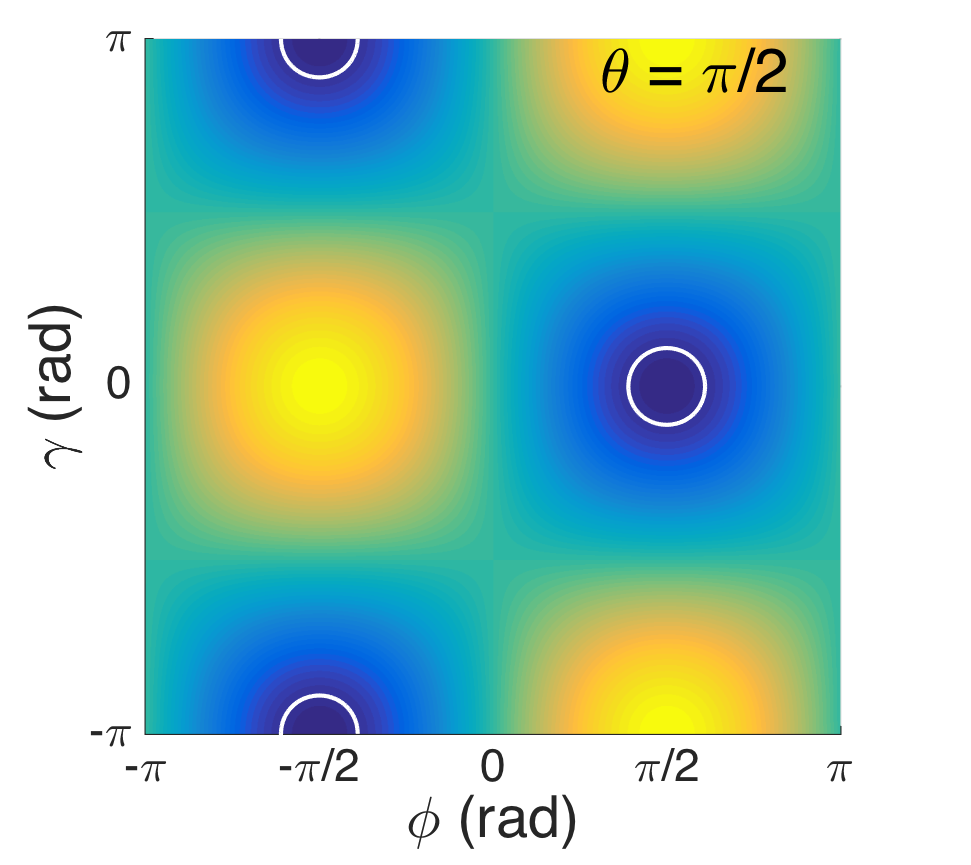
\includegraphics[width=\textwidth]{figs/Figure5a.eps}
%    	\caption{\label{phasea}}
%    \end{subfigure}
%    \begin{subfigure}[t]{0.32\columnwidth}
%    	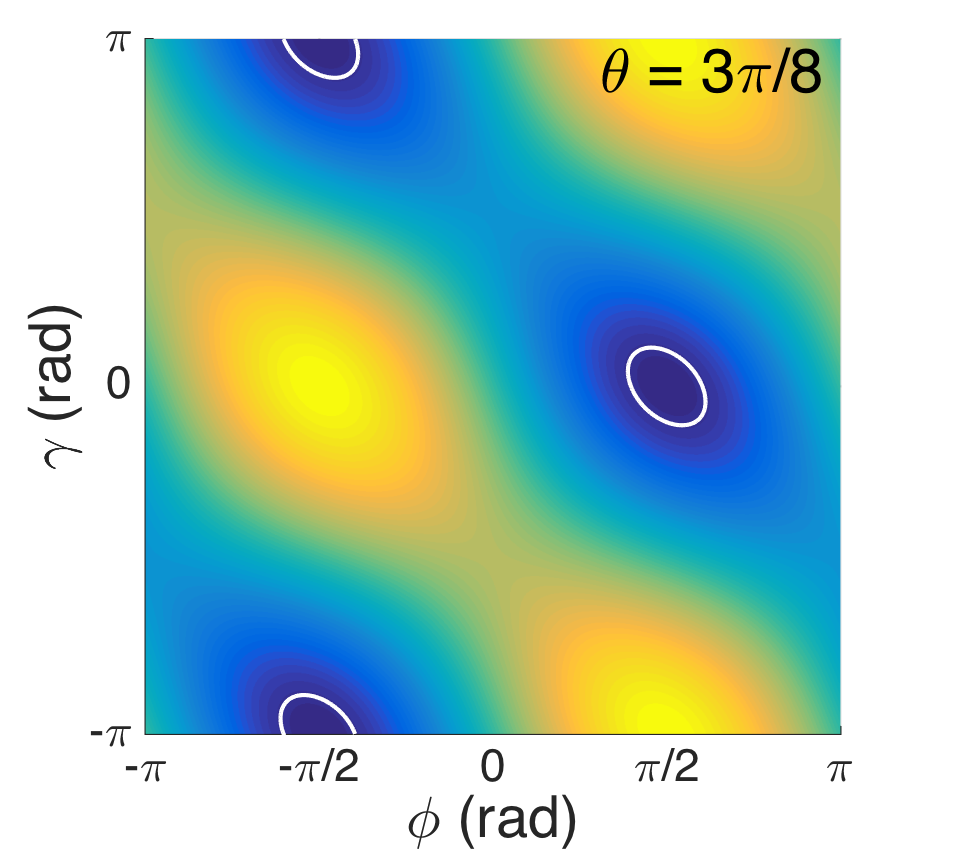
\includegraphics[width=\textwidth]{figs/Figure5b.eps}
%    	\caption{\label{phaseb}}
%    \end{subfigure}
%    \begin{subfigure}[t]{0.32\columnwidth}
%    	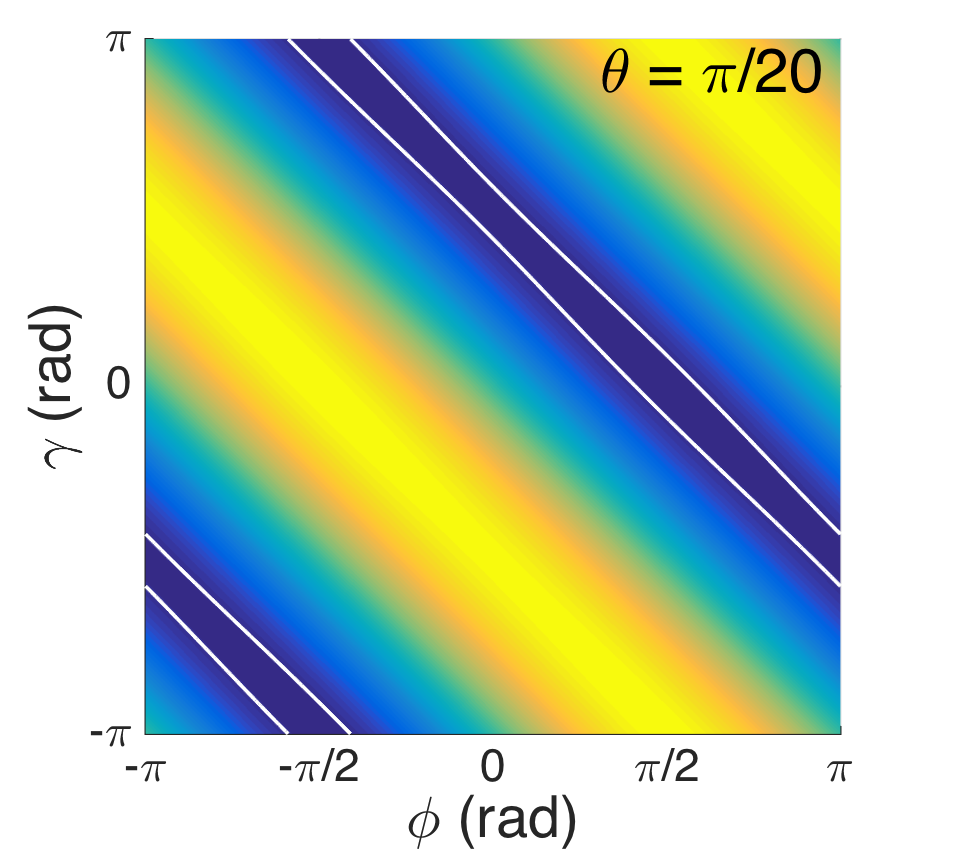
\includegraphics[width=\textwidth]{figs/Figure5c.eps}
%    	\caption{\label{phasec}}
%    \end{subfigure}
\centering
\subfloat[][]{\includegraphics[width=0.5\columnwidth]{figs/Figure4.eps}\label{theorya}}
\subfloat[][]{\includegraphics[width=0.5\columnwidth]{figs/Figure4b.eps}\label{theoryb}} \\
\subfloat[][]{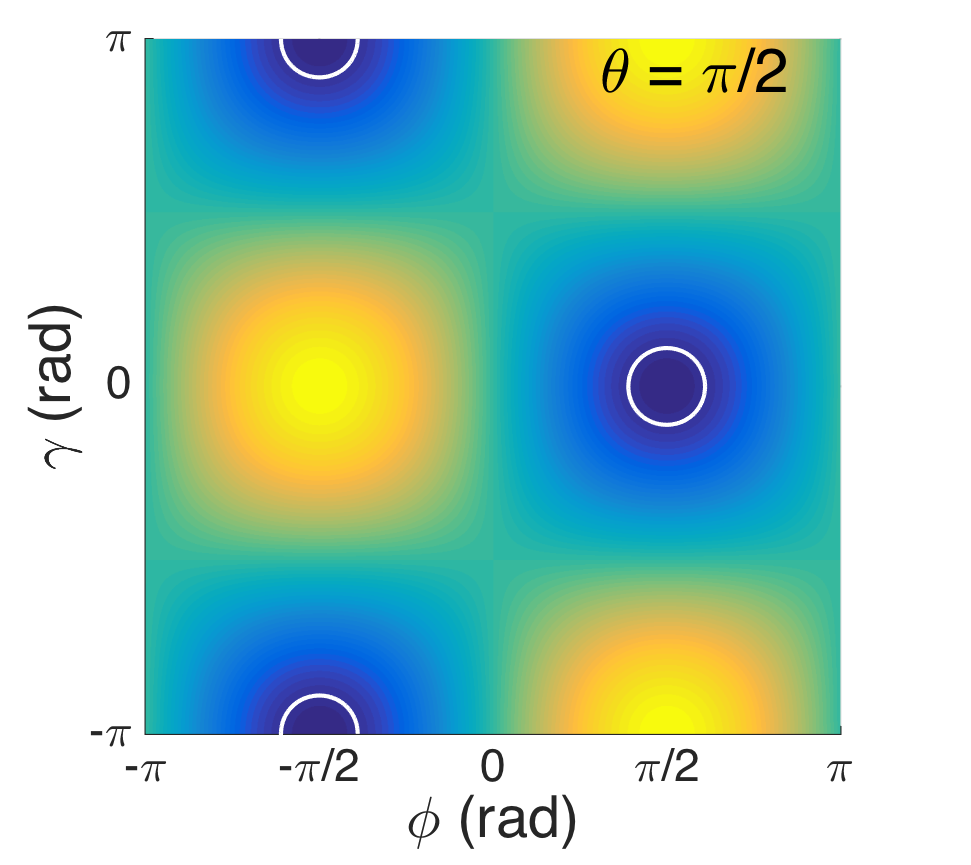
\includegraphics[width=0.33\columnwidth]{figs/Figure5a.eps}\label{phasea}}
\subfloat[][]{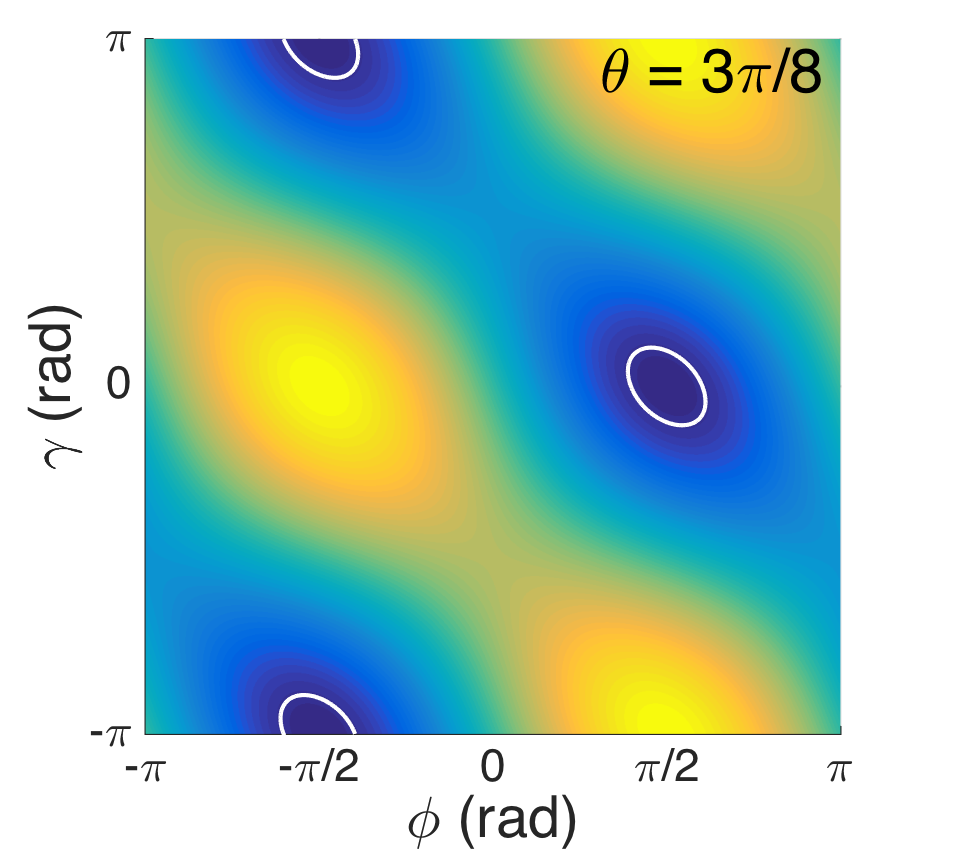
\includegraphics[width=0.33\columnwidth]{figs/Figure5b.eps}\label{phaseb}}
\subfloat[][]{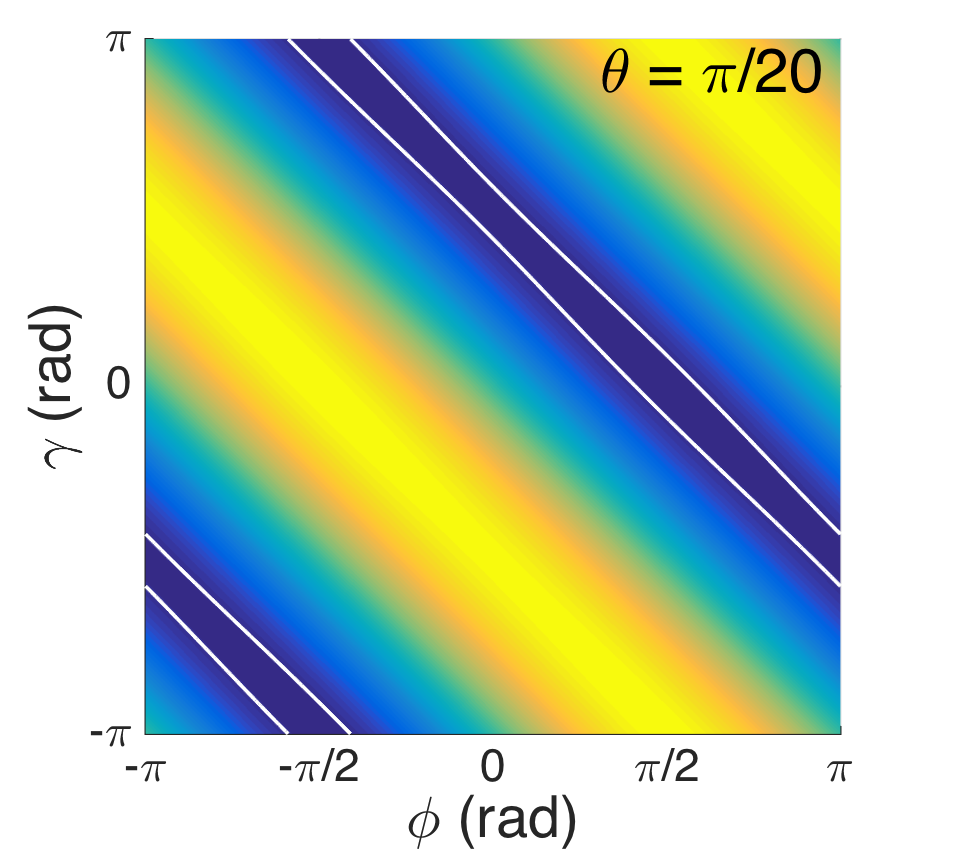
\includegraphics[width=0.33\columnwidth]{figs/Figure5c.eps}\label{phasec}}
    \caption{\footnotesize (a) Probability distribution for a rod with $\mu=1.2 \kk T/G$ in $140$ G (blue) and $0$ G (red) fields shows an emergent bistability between vertical and horizontal states brought on by the external field for an ideal rod (---) and one where $\vc{\mu}$ is offset from the cross-sectional plane by $\epsilon=7^\circ$ (- -). Inset: Relative likelihood ratio between both probability distributions. (b) Same as (a) but for varying magnetic fields. (c-e) The energy $U(\phi,\theta,\gamma)$ for three polar angles $\theta=\frac{\pi}{2},\frac{3\pi}{8},\frac{\pi}{20}$ shows the loss of a degree of freedom. When the rod is lying flat, $\phi$ and $\gamma$ are independently constrained, but when vertical only the sum $\phi+\gamma$ is constrained. This results in the entropic favouring of vertical states compared to intermediate states despite the gravitational cost of standing up. \label{theory}}
\end{figure}

\emph{Discussion.} We wish to interpret the marginal distribution $P(\theta)$. First, we will recap the simpler case whereby two generalised coordinates $(q_1,q_2)$ give rise to a \emph{separable} Hamiltonian $U(q_1,q_2)=U_1(q_1) + U_2(q_2)$. In this case, the natural logarithm of the marginal distribution $P(q_1)$ is: $-\kkT \ln P(q_1) = U_1(q_1) - F_1$, as there is no dependence 

%%%%%%%
Then, setting $\beta=\kk T$ the partition function becomes:

\begin{equation}
Z = \int_{Q_1} \dd q_1\ \ee^{-\beta U_1(q_1)}\int_{Q_2} \dd q_2 \ \ee^{-\beta U_2(q_2)} = Z_1 Z_2.
\end{equation}

This leads to a free energy $F=-\beta^{-1}(\ln{Z_1}+\ln{Z_2}) = F_1 + F_2$. The \emph{marginal} probability distribution over $q_1$ is:

\begin{equation} \label{separable}
P(q_1) = \frac{\ee^{-\beta U_1(q_1)}}{Z} \int_{Q_2} \dd q_2 \ \ee^{-\beta U_2(q_2)} =  \frac{\ee^{-\beta U_1(q_1)}}{Z_1}
\end{equation}

Taking the natural logarithm of both sides and multiplying by $\kk T$ we get:

\begin{eqnarray}
\kk T\ln{P(q_1)} & = & -U_1(q_1) - \kk T\ln(Z_1) \nonumber \\
& = & -U_1(q_1) + F_1.
\end{eqnarray}

Taking expectation values $\kk T \langle \ln{P(q_1)}\rangle_{q_1} = T S_1$ and $\langle U_1\rangle_{q_1}$ gives us the familiar $F_1 = \langle U_1 \rangle - T S_1$. Thus, $-\kk T\ln{P(q_1)}$ and $U_1(q_1)$ differ only by a constant, and so we can interpret $-\kk T\ln{P(q_1)}$ as an energy landscape, where states $\{q_1|q_2=a\}$ which minimise $U_1(q_1)$ are realised more frequently by the system. The question is, how do we interpret the marginal distribution $P(q_1)$, when the energy is \emph{not} composed of separable parts $U_1(q_1)+U_2(q_2)$. In this case, Eq.\ (\ref{separable}) is false, and we have:

\begin{equation}
\kk T\ln{P(q_1)} = \kk T\ln\Big[ \int_{Q_2} \dd q_2 \ \ee^{-U(q_1,q_2)} \Big] - F.
\end{equation}

This is not as readily identifiable as a thermodynamic quantity. However, if we take the (negative) partial derivative with respect to $q_1$, we get:

\begin{eqnarray}
-\kk T\frac{\partial }{\partial q_1} \ln{P(q_1)} & = & \frac{\int_{Q_2} \dd q_2 \ \frac{\partial U(q_1,q_2)}{\partial q_1} \ee^{-U(q_1,q_2)} }{\int_{Q_2} \dd q_2 \  \ee^{-U(q_1,q_2)}}\nonumber \\ 
& = & \Big\langle \frac{\partial U(q_1,q_2)}{\partial q_1} \Big\rangle_{q_2}
\end{eqnarray}

For a rod at an angle $\theta=\Theta$:

\begin{equation} \label{entropicforce}
-\kk T\frac{\partial }{\partial \theta}\Big|_{\theta=\Theta} \ln{P(\theta)}  = \Big\langle \frac{\partial U(\theta,\phi,\gamma)}{\partial \theta}\Big|_{\theta=\Theta} \Big\rangle_{\phi,\gamma}
\end{equation}where the average is taken over the angles $\phi,\gamma$. The right-hand-side of this equation has the form of a force, which we identify as an \emph{entropic} force, meaning that the left hand side is therefore an entropy gradient \emph{[cite Neumann?]}.

Here we are able to reconcile the failure of our intuition. Naively, one would think that for a rod that has found its global energy minimum where $\vc{\mu}$ is aligned along $\vcrm{B}$ while lying flat, the fact that any change in $\theta$ acts only to increase the potential energy ---while leaving $\vc{\mu}\cdot\vcrm{B}$ unchanged--- such a change should be suppressed exponentially. However, Eq.\ (\ref{entropicforce}) tells us that we we must take into account the cost of thermal excursions away from this extremal trajectory. As can be seen from Figs.\ \ref{phasea}-\ref{phasec}, decreasing $\theta$ opens up a larger region of phase-space available to the rod. When the rod is lying flat, $\phi$ and $\gamma$ are independently and tightly constrained such that the rod is confined to a well shown in Fig. \ref{phasea}. In the opposite limit $\theta=0$, only the compound angle $\phi+\gamma$ is defined, opening up a much larger configuration-space available to the rod (this loss of one degree of freedom has the same origin as a gimbal lock in mechanics). Between Figs.\ \ref{phasea} and \ref{phaseb} ($\theta=\pi/2\rightarrow 3\pi/8$), the gravitational energy increases substantially so $P(\theta)$ decays as $\theta$ is decreased. However, between Figs.\ \ref{phaseb} and \ref{phasec} ($\theta=3\pi/8\rightarrow\pi/20$) there is a smaller yet nevertheless positive gravitational cost, but the coinciding gain in available configuration-space is large enough to compensate for this, hence the hopping that we observed experimentally is a true entropy-driven process.

\emph{Conclusions.} It is difficult to draw a quantitative comparison between the data and the theoretical model in most part due to the difficulty of measuring the polar angle of the rod, $\theta$, due to aberrations caused by it standing up out of the focal plane. [\emph{Yongxiang: List 1 or 2 experimental ways to improve this, either in the imaging itself or the image analysis}]. Nevertheless, a significant tendency for the rod to hop to a vertical position is observed in both the projected length $L_p(t)$, and its histogram over all time. Furthermore, both the theoretically predicted likelihood ratio $P(\theta|140 \text{G})/P(\theta|0 \text{G})$ and the same ratio from the data do show good agreement, suggesting that the theory makes a valid explanation of the differential effect of applying the magnetic field. 

Our explanation of this effect highlights some subtle but fundamental physics. The broken axial symmetry due to the perpendicular moment means that when coupled to perpendicular fields ($\vcrm{g}$ and $\vcrm{B}$), the energy is necessarily parameterised by three angles. As such it will suffer the inevitable loss of a degree of freedom when two axes of rotation coincide. This loss results in a reduction in the degree of confinement of the rod and so becomes entropically favourable despite coming at a necessary and substantial energy cost.  Indeed any particle with an orientational energy with broken axial symmetry may be susceptible to this kind of strong entropic effect under the correct temperature conditions.  

\emph{[Some more concluding remarks here].}


%For a rod pivoting about one of its ends, it feels a gravitational torque $\vc{\tau}_g = \frac{m^* L}{2} \hvcrm{n}\times\vcrm{g}$, where $\vcrm{g} = -g\hvcrm{z}$ is the gravitational acceleration. In the presence of an external magnetic field, an additional torque $\vc{\tau}_B = \hvc{\mu}\times\vcrm{B}$ is felt. At $T=290$ K, the characteristic strengths of these torques are $|\vc{\tau}_g| \sim 6 \kk$T, and $|\vc{\tau}_B| \sim\ $0-250$\ \kk$T (for fields in the range of $B=\ $0-120 G)

%\emph{Distribution}


%\section{}
% Put \label in argument of \section for cross-referencing
%\section{\label{}}
%\subsection{}
%\subsubsection{}

% If in two-column mode, this environment will change to single-column
% format so that long equations can be displayed. Use
% sparingly.
%\begin{widetext}
% put long equation here
%\end{widetext}

% figures should be put into the text as floats.
% Use the graphics or graphicx packages (distributed with LaTeX2e)
% and the \includegraphics macro defined in those packages.
% See the LaTeX Graphics Companion by Michel Goosens, Sebastian Rahtz,
% and Frank Mittelbach for instance.
%
% Here is an example of the general form of a figure:
% Fill in the caption in the braces of the \caption{} command. Put the label
% that you will use with \ref{} command in the braces of the \label{} command.
% Use the figure* environment if the figure should span across the
% entire page. There is no need to do explicit centering.

% \begin{figure}
% \includegraphics{}%
% \caption{\label{}}
% \end{figure}

% Surround figure environment with turnpage environment for landscape
% figure
% \begin{turnpage}
% \begin{figure}
% \includegraphics{}%
% \caption{\label{}}
% \end{figure}
% \end{turnpage}

% tables should appear as floats within the text
%
% Here is an example of the general form of a table:
% Fill in the caption in the braces of the \caption{} command. Put the label
% that you will use with \ref{} command in the braces of the \label{} command.
% Insert the column specifiers (l, r, c, d, etc.) in the empty braces of the
% \begin{tabular}{} command.
% The ruledtabular enviroment adds doubled rules to table and sets a
% reasonable default table settings.
% Use the table* environment to get a full-width table in two-column
% Add \usepackage{longtable} and the longtable (or longtable*}
% environment for nicely formatted long tables. Or use the the [H]
% placement option to break a long table (with less control than 
% in longtable).
% \begin{table}%[H] add [H] placement to break table across pages
% \caption{\label{}}
% \begin{ruledtabular}
% \begin{tabular}{}
% Lines of table here ending with \\
% \end{tabular}
% \end{ruledtabular}
% \end{table}

% Surround table environment with turnpage environment for landscape
% table
% \begin{turnpage}
% \begin{table}
% \caption{\label{}}
% \begin{ruledtabular}
% \begin{tabular}{}
% \end{tabular}
% \end{ruledtabular}
% \end{table}
% \end{turnpage}

% Specify following sections are appendices. Use \appendix* if there
% only one appendix.
%\appendix
%\section{}

% If you have acknowledgments, this puts in the proper section head.
%\begin{acknowledgments}
% put your acknowledgments here.
%\end{acknowledgments}

% Create the reference section using BibTeX:
\bibliography{refs/refs.bib}

\end{document}
%
% ****** End of file apstemplate.tex ******

